\section{Regularización}

La última técnica a usar en este texto es la técnica de regularización, esta es usada para librarnos de dos problemas al momento de entrenar. Estos problemas son el \textit{sobre ajuste} y el \textit{ajuste pobre}, en inglés \emph{overfitting} y \emph{underfitting} respectivamente.

Recordemos que dado un problema de aprendizaje, se define un espacio de hipótesis, es decir, una familia de posibles funciones que vamos a utilizar para encontrar la función objetivo, que queremos aproximar. 

El espacio de hipótesis puede ser tan grande o tan pequeño como la cantidad de funciones que estén contenidas en él. Así tenemos dos situaciones:
\begin{itemize}
 \item Si el espacio de hipótesis, no contiene a la función objetivo, entonces por más que ejecutemos los algoritmos de entrenamiento, no va a ser posible llegar a una buena aproximación.
 \begin{example}
  Si la función objetivo tiene la forma de una parábola, y únicamente la intentamos aproximar con funciones lineales, es claro que nunca vamos a dar una buena aproximación.
 \end{example}

 \item Si el espacio de hipótesis, es demasiado gigantesco, podemos llegar a tener problemas encontrando la respuesta correcta. 
\end{itemize}

Las dos situaciones anteriores nos llevan a los dos problemas antes mencionados:
\begin{description}
 \item [Ajuste pobre] 
 Cuando un modelo, no logra reducir suficientemente el error sobre el conjunto de entrenamiento (menos aún sobre el de validación) ver \fref{fig:underF}.
  \begin{figure}[H]
   \centering
   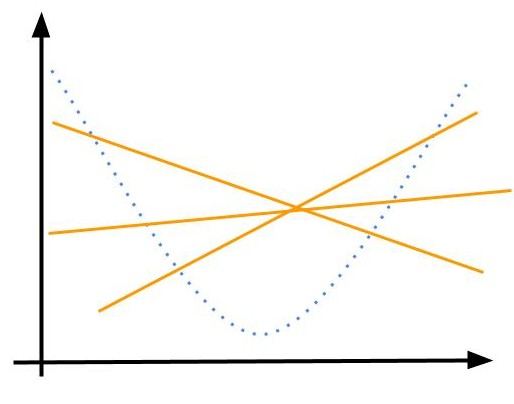
\includegraphics[scale=0.5]{../Figuras/underfitting.jpg}
   \caption{Ejemplo de ajuste pobre. La línea punteada es la función objetivo, las líneas naranjas el espacio de hipótesis.}
   \label{fig:underF}
  \end{figure}

 \item [Sobre ajuste]
 Cuando un modelo, reduce muy bien el error con el conjunto de entrenamiento, pero con el conjunto de validación el error es muy alto, es decir, la hipótesis no generaliza a datos no vistos previamente, ver \fref{fig:overF}.
 \begin{example}
  Los datos del entrenamiento asemejan la función de un polinomio, entonces la red aprende solo a identificar los datos que pasen por la función, al momento de agregar datos nuevos estos probablemente nos se comporten conforme al polinomio y nunca los clasifique adecuadamente. 
 \end{example}

  \begin{figure}[H]
   \centering
   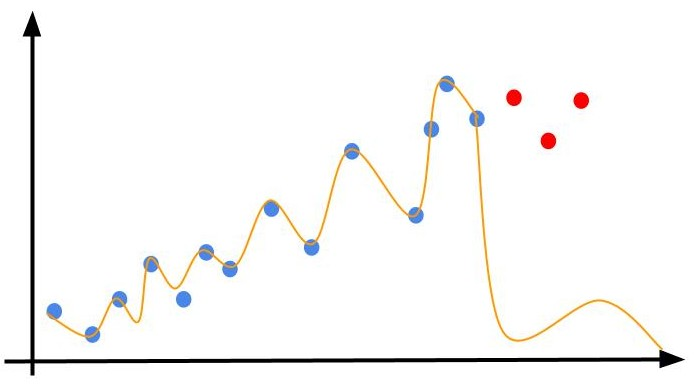
\includegraphics[scale=0.5]{../Figuras/overfitting.jpg}
   \caption{Ejemplo de sobre ajuste. La función aproximada de color naranja. Los datos durante el entrenamiento de color azul. Los datos nuevos de color rojo.}
  \label{fig:overF}
  \end{figure}
 \end{description}

Estos dos problemas puden suceder por dos razones distintas:
\begin{enumerate}
 \item La cantidad de neuronas, dos casos:
    \begin{itemize}
     \item \textbf{Faltan neuronas}: El espacio de hipótesis es muy simple para poder aproximar la función, es decir, tenemos un \textit{ajuste pobre}.
    
    \item \textbf{Sobran neuronas}: El espacio de hipótesis es muy expresivo. No obtiene las características de la función objetivo, sino que memorizó las etiquetas de los datos de entrada, es decir, tenemos un \textit{sobreajuste}.
    \end{itemize}

 \item Faltan datos de entrenamiento, entonces independientemente del número de neuronas, el error en los datos de validación no baja, o incluso ni en los datos del entrenamiento.
\end{enumerate}

Cuando nos sobran nueronas lo podemos detectar, porque al reducir neuronas, el desempeño de la red entrenada en el conjunto de entrenamineto, no empeora significativamente, y el desempeño con los datos de validación mejora.

En este caso lo que vamos a hacer es modificar la función de pérdida la nueva función va a estar integrada por dos componentes por un lado la función de error que ya teníamos aquí debo aclarar que yo estoy utilizando libremente función de pérdida función de error y ustedes van a encontrar en la literatura que se intercambian estos dos nombres tranquilamente yo prefiero ahorita enfatizar de momento que la función de error es la que mide tal cual la distancia entre los valores obtenidos y los valores que queríamos y el segundo término ya no tiene nada que ver con esto el segundo término es una penalización sobre las magnitudes de los pesos de la red los a la suma de estos dos es lo que estoy llamando función de pérdida pero insisto esta fue una elección personal no necesariamente la van a encontrar igual en otros lados bueno si consideramos estas dos cosas entonces la función que estamos tratando de minimizar es esta que es la suma de estas dos y el efecto que va a tener si es el siguiente el mínimo de esta función hallará un punto de compromiso tal que reduce el error lo más posible dejando crecer solamente aquellos pesos que contribuyan mejor a reducir el error compensando por la contribución de su magnitud creciente es decir ahora tenemos una red en la cual colocamos desde el inicio muchas neuronas lo cual naturalmente tendería a producir una obra y ting pero lo que vamos a hacer es penalizar los pesos de manera que solita el algoritmo de optimización haga que solamente aquellas conexiones que realmente están contribuyendo a reducir el error tengan magnitudes significativas aquellas conexiones que no contribuyan entenderán entonces a tener magnitudes muy pequeñas y por consiguiente ser casi casi como si no estuvieran ahí es como una manera de hacer que nuestro algoritmo de optimización o de un poco nuestra red neuronal y haga que algunas de las conexiones queden muy muy débiles y básicamente ya no contribuyan entonces la hipótesis que se va a aprender va a ser éste mucho más sencilla y la idea es que esto logre capturar mejor la función que estamos tratando de aproximar en lugar de memoriza estilos ahora igual que en el caso anterior dependiendo de qué tan rigurosos seamos con esta penalización podemos hacer que las únicas conexiones que pueden subir su magnitud en realidad muy poquitas y también podría darse el problema de under fighting entonces también no nos libramos de tener que calibrar un poquito este parámetro extra que va a provocar la penalización entonces vamos a tener una gráfica un poco parecida a la de antes e igualmente cómo se va a ver la edición de este error bueno aquí vemos que del lado izquierdo tenemos nuestra función de error podría ser una entropía cruzada podrían ser diferencias cuadrado o alguna otra que nos llegamos a encontrar nos resulte útil para nuestro problema el segundo término va a ser precisamente esta penalización aquí estoy poniendo la más común que es simplemente sumar los todos los cuadrados de las magnitudes de todos los pesos que tienen la red es un término muy sencillo que va a provocar que esta función suba de valor si estamos utilizando esos con magnitudes grandes entonces la manera de minimizar la es solamente dejando subir los valores y aquellos pesos que ayuden a compensar bajando el nivel de penalización entonces está regido por este parámetro lambda entre más grande sea lambda observen que más se va a incrementar el valor de esta función por culpa de los pesos entonces este término se va a volver mucho más importante el cálculo del error si la lambda es muy pequeña entonces el término dominante va a ser la función original de error y va a haber muy poquita penalización muy poco efecto por el hecho de haberle subido la magnitud de los pesos por consiguiente vamos a obtener una gráfica equivalente a la que teníamos anteriormente pero ahora en términos del parámetro lambda observemos que cuando el lambda es 0 tenemos la función de error original esto equivaldría a tener nuestra red neuronal con el montón de neuronas que le pusimos no hay penalización y podríamos tender precisamente al problema de over fitting entonces vemos la perfil de este lado donde el error en el entrenamiento es muy bajo pero en el conjunto de validación es muy malo es decir nuestra red no sabe predecir después en el otro extremo es cuando estamos penalizando tanto por los pesos que ya nuestro algoritmo de optimización pues lo que hizo fue encoger pesos y casi casi no se ocupó de corregir el error entonces tenemos acá un under fitting realmente nuestra red casi casi no pudo participar y no está modelando bien nuestra función entonces tenemos un error bastante alto y bueno la función de validación también está creciendo el el error no las predicciones tampoco tan bueno y en algún lugar de por en medio vamos a tener un compromiso interesante entre la habilidad para predecir creo que aquí es donde están varias predicciones bueno el error en el conjunto de entrenamiento a lo mejor aquí se podría más o menos por esta zona estaría en nuestro punto óptimo entonces podemos hacer también esta gráfica y tratar de identificar en qué punto estamos obteniendo la mejor red posible básicamente es ley. 
